\documentclass[a4paper,10pt]{article}
\usepackage[utf8]{inputenc}
\usepackage[spanish]{babel}
\usepackage[affil-it]{authblk}
\usepackage{enumerate}
\usepackage{graphicx}
\usepackage{hyperref}
\usepackage{amsmath}
\usepackage{amssymb}
\usepackage{cancel}
\usepackage{tikz}
\usepackage{cleveref}
\usetikzlibrary{calc}
\numberwithin{equation}{section}

%Multiple References

\usepackage{xparse}
\ExplSyntaxOn
\NewDocumentCommand{\mref}{m}{\quinn_mref:n {#1}}
\seq_new:N \l_quinn_mref_seq
\cs_new:Npn \quinn_mref:n #1
 {
  \seq_set_split:Nnn \l_quinn_mref_seq { , } { #1 }
  \seq_pop_right:NN \l_quinn_mref_seq \l_tmpa_tl
  ( % print the left parenthesis
  \seq_map_inline:Nn \l_quinn_mref_seq
    { \ref{##1},\nobreakspace } % print the first references
  \exp_args:NV \ref \l_tmpa_tl 
  ) 
 }
\ExplSyntaxOff


%Boxes

\newcommand*{\boxcolor}{blue}
\makeatletter
\renewcommand{\boxed}[1]{\textcolor{\boxcolor}{%
\tikz[baseline={([yshift=-1ex]current bounding box.center)}] \node [rectangle, minimum width=1ex,rounded corners,draw] {\normalcolor\m@th$\displaystyle#1$};}}
 \makeatother

%Constantes
\newcommand{\euler}{\mathrm{e}}
\newcommand{\im}{i}

%opening
\title{Mecánica Clásica Tarea \# 3}
\author{Favio Vázquez\thanks{Correo: favio.vazquezp@gmail.com}}\affil{Instituto de Ciencias Nucleares. Universidad Nacional Autónoma de México}
\date{}

\begin{document}

\makeatletter
\def\@maketitle{%
  \newpage
  \null
  \vskip 2em%
  \begin{center}%
  \let \footnote \thanks
    {\Large\bfseries \@title \par}%
    \vskip 1.5em%
    {\normalsize
      \lineskip .5em%
      \begin{tabular}[t]{c}%
        \@author
      \end{tabular}\par}%
    \vskip 1em%
    {\normalsize \@date}%
  \end{center}%
  \par
  \vskip 1.5em}
\makeatother

\maketitle

\section{Problema 1}

Trace el diagrama o retrato de fase que corresponde al movimiento de una
partícula en una dimensión sujeta al potencial que se ilustra en la 
figura.

\begin{figure}[h]
 \center 
 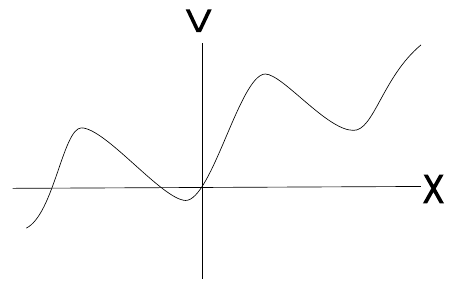
\includegraphics[scale=0.5]{problema1fig1}
 \caption{Problema 1. Diagrama del potencial a estudiar}
\end{figure}

\vspace{.3cm}

\underline{Solución:} \vspace{.3cm}

\section{Problema 2}

Demuestre que una trayectoria de Lissajous en el espacio físico de dos 
dimensiones cubre densamente la región a la que tiene acceso si, y sólo si,
las dos frecuencias son inconmensurables.

\vspace{.3cm}

\underline{Solución:} \vspace{.3cm}

\section{Problema 3}

Encuentre la sección de dispersión para un potencial coulombiano repulsivo.

\vspace{.3cm}

\underline{Solución:} \vspace{.3cm}

\section{Problema 4}

Demuestre que una partícula moviéndose en una dimensión y sujeta a la 
acción de una fuerza 

$$ 
f = -kx^{2n+1} \qquad n \quad \text{entero positivo,}
$$

oscilará con un período proporcional a $A^{-n}$, donde $A$ es la amplitud 
de la oscilación. ¿Es esto válido cuando $n<0$?

\vspace{.3cm}

\underline{Solución:} \vspace{.3cm}

\section{Problema 5}

Grafique las proyecciones $(\theta,r)$, $(\theta,\dot{r})$, $(r,\dot{r})$,
y $(r,\dot{\theta})$ en el espacio de fase $(\theta,r,\dot{\theta},\dot{r})$
(ojo no se trata dela órbita) de una partícula sujeta a una fuerza central 
gravitacional. Considere tanto casos con energía total positiva, como 
negativa.

\vspace{.3cm}

\underline{Solución:} \vspace{.3cm}


\end{document}
